\section{Challenge II: Building an Efficient Body Movement Based Authentication System}\label{sec:system}


The second challenge we will deal with in this project is to ensure the proposed authentication system can run on seriously resource-constrained wearable devices. Our preliminary results show that even a highly simplified classifier will incur high processing latencies, sometimes leading to the catastrophic device overheat exception. To tackle this challenge, we propose to carefully select efficient features and classifiers, pipeline the authentication operations, and dynamically adapt the sampling rate.

\subsection{Preliminary Work}
\begin{wrapfigure}{r}{3.0in}\vspace{-12pt}
\centering
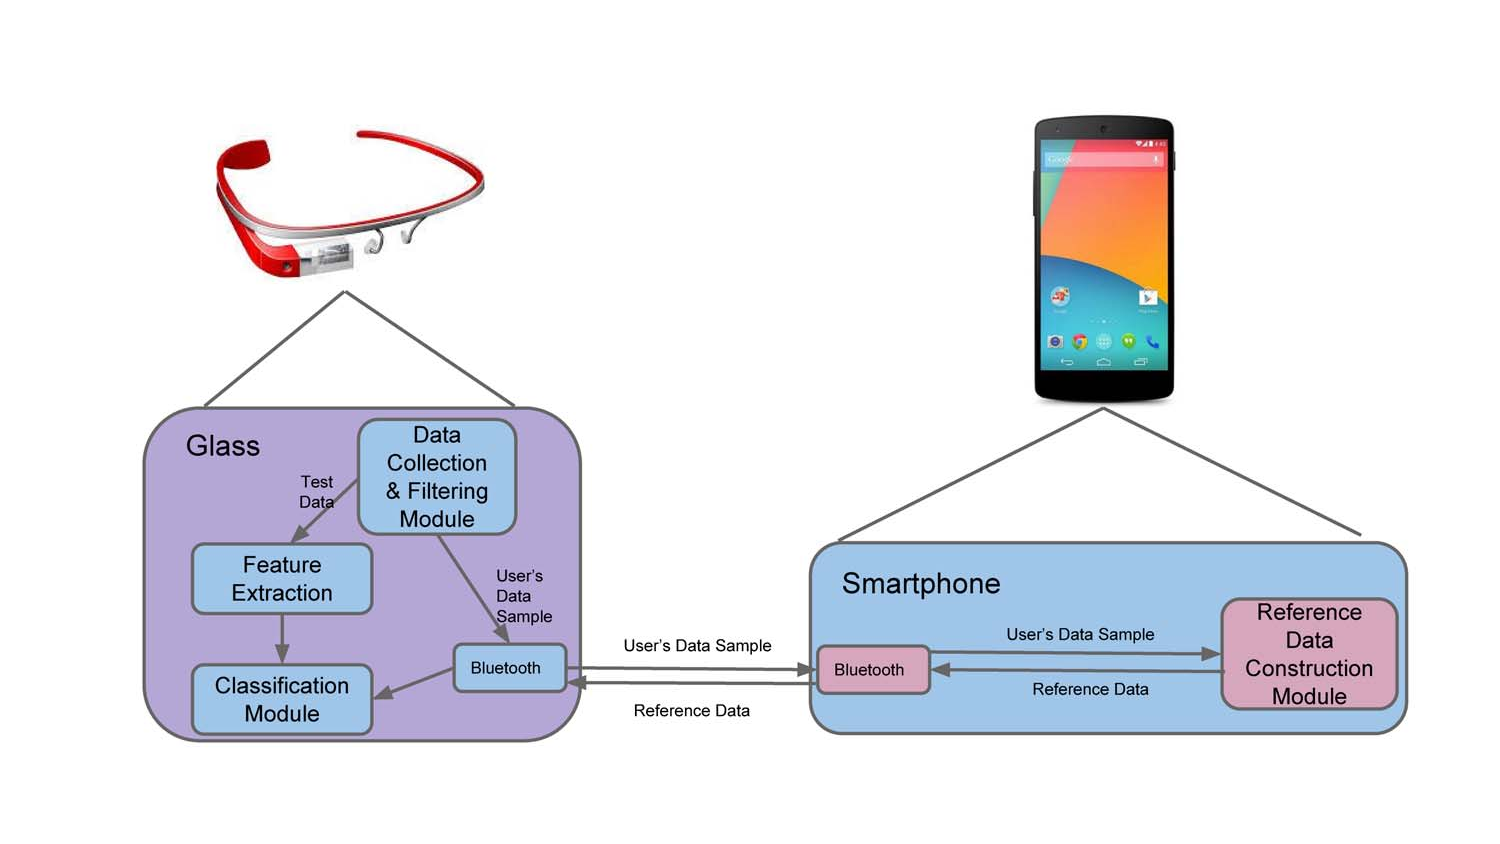
\includegraphics [width=.9\linewidth]{../figure/sofware_architecture}
\caption{The software modules for the Headbanger authentication app we implemented in the preliminary study. \label{fig:software_arch}}\vspace{-12pt}
\end{wrapfigure}
Wearable devices have severe resource limitations in many aspects; to name a few, energy, computing, networking and storage. Building an efficient authentication system that can smoothly run on such devices, therefore, becomes a significant challenge. In order to investigate whether such a goal is attainable, we have implemented a ~\systemname~app on the Google Glass. Figure~\ref{fig:software_arch} shows the software modules the app consists of. In the implementation, we established the reference data on the smartphone since this step is offline, consumes the most resources, and doesn't need to run on the device. The online
authentication process is implemented on the device. In the implementation, we adopted a much simplified classification method. First, instead of having multiple reference samples, we only use one reference sample for each user. After computing the DTW distance between the test sample and the reference sample, we simply compare the distance to a pre-set threshold value to determine the classification result. In this implementation, we kept the algorithm to the bare minimum to test the processing capability of the Google Glass and did not worry about the classification accuracy.

\begin{wrapfigure}{r}{3.0in}\centering
\small\centering
\begin{tabular}{|l|l|}\hline
sample  & processing \\
duration (s) & delay (s) \\\hline
2 & 1.29 \\\hline
3 & 2.74 \\\hline
6 & 9.04 \\\hline
10 & 20.48 \\\hline
\end{tabular}
\caption{\label{tab:glass}Measured processing latencies on Google Glass with different sample durations. In this set of experiments, we tried to understand the processing capability constraints and didn't optimize the code. }
\end{wrapfigure}
Figure~\ref{tab:glass} shows the measured processing latency (the time that elapsed between when we finish collecting the test sample and when the authentication result is generated). The results show that even with a significantly reduced implementation, the processing delays are still rather substantial. For example, if the sample duration is 10 seconds, the processing delay is a little more than 20 seconds! More importantly, if there were other processes such as camera running at the same time, or if we continuously ran the~\systemname~app for multiple times, then the processing became very slow, and the glass became overheated and displayed the following message ``It is too hot. Glass needs to cool down.'' Then we needed to wait for 1 or 2 minutes for the glass to cool down. After the glass finally cools down, we had to start over the authentication process from the beginning. We refer to this catastrophic event as \emph{glass overheat exception}.

From the preliminary investigation, it becomes very natural that the second research challenge we have to address in this project is to optimize the system design of~\systemname~to enable efficient execution on severely resource-constrained wearable devices.

